\documentclass{article}
\usepackage{fullpage}
\usepackage{times}
\usepackage{fancyhdr,graphicx,amsmath,amssymb}
\usepackage[ruled,vlined]{algorithm2e}
\include{pythonlisting}

\usepackage{multirow}
\usepackage{graphicx}
\usepackage{blindtext}
\usepackage{subcaption}
\usepackage{arxiv}
\usepackage{listings}
\lstset
{ %Formatting for code in appendix
    language=C,
    basicstyle=\footnotesize,
    numbers=left,
    firstnumber= 0,
    stepnumber=1,
    showstringspaces=false,
    tabsize=1,
    breaklines=true,
    breakatwhitespace=false,
    xleftmargin=0.04\textwidth,
}
\usepackage[utf8]{inputenc} % allow utf-8 input
\usepackage[T1]{fontenc}    % use 8-bit T1 fonts
\usepackage{hyperref}       % hyperlinks
\usepackage{url}            % simple URL typesetting
\usepackage{booktabs}       % professional-quality tables
\usepackage{amsfonts}       % blackboard math symbols
\usepackage{nicefrac}       % compact symbols for 1/2, etc.
\usepackage{microtype}      % microtypography
\usepackage{lipsum}
\newcommand*\samethanks[1][\value{footnote}]{\footnotemark[#1]}
\newcommand{\tabincell}[2]{\begin{tabular}{@{}#1@{}}#2\end{tabular}}
\title{Systematic Predicate Abstraction using Deep Learning}


\author{
  Name \thanks{All contributions are considered equal.}\\
  Department of \\
   University\\
  Address \\
  \texttt{xxx@xxx} \\
  %% examples of more authors
   \And
 Name \samethanks\\
  Department of \\
   University\\
  Address \\
  \texttt{xxx@xxx} \\
     \And
 Name \samethanks\\
  Department of \\
   University\\
  Address \\
  \texttt{xxx@xxx} \\
  %% \AND
  %% Coauthor \\
  %% Affiliation \\
  %% Address \\
  %% \texttt{email} \\
  %% \And
  %% Coauthor \\
  %% Affiliation \\
  %% Address \\
  %% \texttt{email} \\
  %% \And
  %% Coauthor \\
  %% Affiliation \\
  %% Address \\
  %% \texttt{email} \\
}

\begin{document}
\maketitle

\begin{abstract}
Systematic Predicate Abstraction using Deep Learning
\end{abstract}


% keywords can be removed
\keywords{First keyword \and Second keyword \and More}


\section{Introduction}
Systematic Predicate Abstraction using Deep Learning




\subsection{Problem overview and working pipeline}

Our purpose is to find better predicates that can represent correct abstract transition system by a learned heuristic. In CEGAR iteration, the predicates come from two sources. One is initial predicates that can be generated by some heuristics before the first iteration [cite]. Another is the predicates generated from counter-examples after the first iteration. We can add an heuristic to generate better predicates in both situations. The heuristic is the importance of arguments. It can be represented by counting the number of occurrence of arguments in predicates.

In the case of verifiable programs, we expect the learned heuristic can reduce CEGAR iterations or total time consumption for verifying the program. In the case of unverifiable programs (cannot verify the program within a fixed time), we expect the learned heuristic can help Eldarica to verify it.


The working pipeline is:
\begin{enumerate}
  \item Collect training inputs: Feed verifiable programs to Eldarica. Eldarica transforms the program to horn clauses and horn graphs. Eldarica uses current heuristic to solve the horn clauses. During the CEGAR process, some predicates are generated.
  \item Collect training labels: In in generated predicates, count the number of occurrence of arguments appeared in horn clauses to be the training labels.
  \item Train a model: A GNN + multilayer perceptrons model is built and trained. The input is horn graph, the output is the number of occurrence of arguments.
  \item Apply trained model: For one program, apply Eldarica to transform the program to horn graph and feed it to the trained model. The output is the number of occurrence (i.e. importance) of arguments.
  \item Apply predicted results: Use the output as a heuristic to start a CEGAR process to solve the horn clauses transformed from the program by Eldarica.
\end{enumerate}



\subsection{Contribution}

\begin{itemize}
  \item We define horn graph which captures control flow and data flow in horn clauses. The semantics and syntaxes of the program is preserved as much as possible. Horn graph bridges horn clauses and graph related analysis and learning methods.
  \item We provides a way to build a interface that take horn clauses as inputs and node features or graph representation as output for deep learning tasks based on horn clauses.
  \item We extend GNN to handle hyperedges
  \item Experiment results give confidence that
\end{itemize}

\section{Background}
\subsection{Abstraction Based Model Checking}
Model checking is a technique for program verification. It builds a transition system based on variables' states in all control locations and to check if there is a path to the error states. The error states are built by specifications given by users. But, programs with infinite states are ubiquitous. Therefore, we need to find a finite transition system (abstract transition system $\widehat{M}$) to represent the infinite transition system $M$, such that if there is no path to the error state in $\widehat{M}$, $M$ has no error as well, and if there is a path to the error state in $\widehat{M}$, we can use this concrete error path to check if there is a error in $M$.

The major challenge in this idea is to find a appropriate $\widehat{M}$. CEGAR \cite{10.1007/10722167_15} is a state-of-art framework to find $\widehat{M}$ iteratively. CEGAR framework is described in Figure \ref{CEGAR}. It starts with a initial abstract transition system $\widehat{M}$. The model checker can check if there is a path to the error state. If there is no such path, the the system $M$ is safe, otherwise give the path as a counterexample to check the feasibility. Checking feasibility means to use this counterexample as input to $M$ If $M$ return a error, this counterexample is feasible and $M$ is not safe. If there is no error returned, this counterexample is infeasible which means $\widehat{M}$ does not represent $M$. Therefore, we need a new abstract transition system $\widehat{M}'$ obtained by a refinement process.

\begin{figure}[h]
\centering
  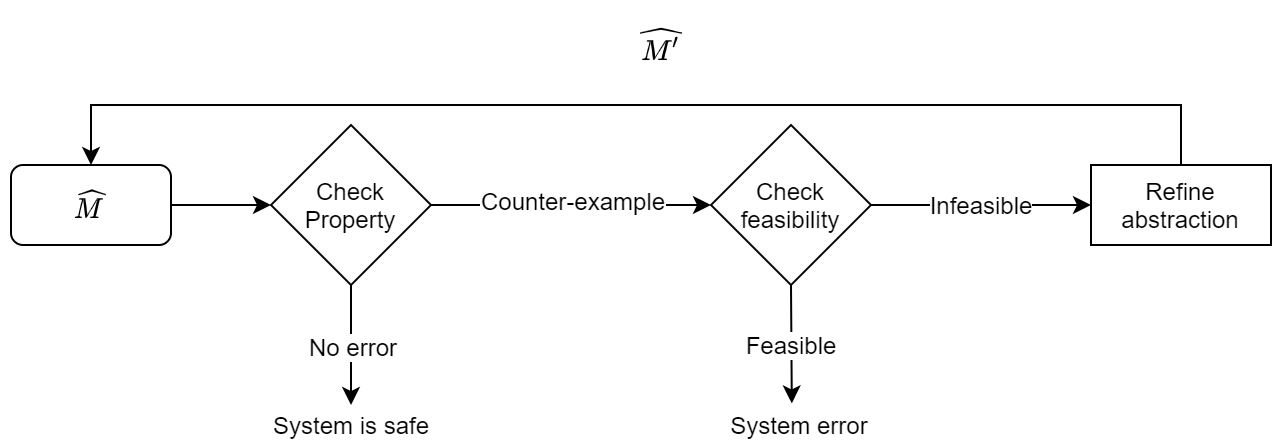
\includegraphics[width=12cm]{graph/CEGAR}\\
  \caption{CEGAR framework}\label{CEGAR}
\end{figure}


$\widehat{M}$ is built by a set of predicates $P$. To update $\widehat{M}$ to $\widehat{M}'$ means to update $P$ to a new predicate set $P'$ by adding new predicates. The new predicates are constructed by splitting the counterexample path to two parts $A$ and $B$ and find the Interpolants $I$ of $A$ and $B$, such that $I$ consists of common elements in $A$ and $B$, $A\Rightarrow I$, and $I\Rightarrow$ $\neg B$. $I$ is the new predicates to be added to $P$.

\subsubsection{Heuristics for predicate generating}
---
%\subsection{Abstract Interpolation}
Abstract Interpolation \cite{10.1007/978-3-319-57288-8_18}.

Manually constructed templates \cite{10.1007/978-3-319-57288-8_18}

Learned argument importance as heuristic.

\subsection{GNN}
The program is transformed to horn graph which preserves the structural information of the graph by catching control flow and data flow. We apply tf2\_gnn framework to learn the node features from graph inputs. tf2\_gnn is a implementation of general GNN framework which provides standard inputs and outputs for graph learning. Except implementing several popular GNN algorithms, such as \cite{2017arXiv171010903V,schlichtkrull2017modeling}, it also provides great flexibility to implement customized GNNs. The inputs of tf2\_gnn is node vector and edges which represent the relations between node vectors. The output can be node features or a graph feature. Since we want to learn the importance of arguments. We take node features as outputs. We gather these learned argument node features and apply multilayer perceptrons to learn the importance of them.

\subsubsection{Message passing and hyperedge extension}
---





\section{Program representation}
Our raw inputs are programs in text format and could be written in different languages. We first transform programs to horn clauses which can preserve the semantics. We perform learning process in Horn clauses level. In this way, we can eliminate the affects from different program languages.


But, Horn clauses are also in text format and text-level embedding methods \cite{mikolov2013efficient} are not enough to capture the structural information. The downstream multilayer perceptron cannot learn well from the text-level embedding. Therefore, we transform Horn clauses to graph format which contains both control flow and data flow information that capture the structure information from Horn clauses, then we use GNN to learn the representation of the horn graph to be the representation of the original program.


\subsection{Program to Horn clauses}
Eldarica can transform SMT or C format programs to intermediate horn clause format and the semantics are preserved [cite].  By using horn clauses as the learning inputs, we don't need to care about the input languages but focus on solving the logic problems. We have an example in Figure \ref{while-C-program} and \ref{while-C-horn-clauses} to explain how to transform c program to horn clauses and preserving semantics.

In Figure \ref{while-C-program}, we have a simple while loop C program which assumes variable $x$ and $y$ equal to external input Integer $n$ and $n\geq 0$. The assertion is $y==0$. The corresponding Horn clauses are described in  Figure \ref{while-C-horn-clauses}. Every line is consists of $Head:-Body,[constraint]$. For example, in line 0, $Head$ is $inv\_main4(x, y)$ which means in control location $while(x!=0)$ in the main function, there are two variables $x$ and $y$. $Body$ is empty here because this is the initial state of the program. The $constraint$ is $n \geq 0 \wedge x = n \wedge n = 0 \wedge y = n$ which comes from the $assume(x==n\&\&y==n\&\&n>=0)$ in the C program. Line 0 means in control location $while(x!=0)$, there are two variables $x$, and $y$, which satisfy the $constraint: n \geq 0 \wedge x = n \wedge n = 0 \wedge y = n$. In line 1, The body is not empty, this means that there is a transition from body to head and this transition satisfy the $constraint$. Line 1 means from control location $while(x!=0)$ to next iteration, it must satisfy that, $x!=0$ and in the new iteration, the variables $arg1$ and $arg2$ in the control location $while(x!=0)$ must equal to $x-1$ and $y-1$, (values of $x,y$ come from last iteration). Line 2 transforms the semantic of assertion $y==0$ to horn clauses. Line 2 means that from control  location $while(x!=0)$ to false state, in the control location $while(x!=0)$ , the variable $x$ is 0 and $y$ satisfy $y!=0$.


\begin{figure}[h]
\begin{subfigure}[b]{0.4\textwidth}
\begin{lstlisting}
extern int n;
void main(){
    int x,y;
    assume(x==n&&y==n&&n>=0);
    while(x!=0){
        x--;
        y--;
    }
    assert(y==0);
}
\end{lstlisting}\subcaption{An input example: C program}\label{while-C-program}
\end{subfigure}
\begin{subfigure}[b]{0.6\textwidth}
\begin{lstlisting}
inv_main4(x, y) :- ,[n >= 0 & x = n & 0 = n & y = n].
inv_main4(arg1, arg2) :- inv_main4(x, y), [x != 0 & x + -1 = arg1 & y + -1 = arg2 & n = 0].
false :- inv_main4(0, y), [y != 0].
\end{lstlisting}\subcaption{Horn clauses for C program}\label{while-C-horn-clauses}
  \end{subfigure}
  \caption{}
\end{figure}

How to transform program in c or smt2 format to horn clauses and why the sematic can be preserved can be found in [cite]. Our main purpose is to use this horn clauses format as input of deep learning structure to perform downstream tasks.
%to select better templates to reduce the number of iterations in CEGAR loop.


\subsection{Horn clauses to Horn graph}
As we mentioned before, horn clauses in text format is hard to learn the structure information. Therefore, we need transform horn clauses to horn graph.
We defined a way to construct Horn graph from Horn clauses, which preserves syntactical and sematic information as much as possible. This definition is not unique, one can define their own horn graph.

We first provided an example that transform horn clauses in Figure \ref{while-C-horn-clauses} to horn graph in Figure \ref{overall-transformation}.
Then, we give formal definition of our horn graph construction process.

\subsubsection{Horn graph construction example} \label{Horn-graph-construction-example}
The graph is constructed by parsing the horn clauses line by line. In Figure \ref{while-C-horn-clauses}, every line is a horn clause. In , Line 0 "inv\_main4(x, y) :- ,[n >= 0 \& x = n \& 0 = n \& y = n]", the left hand side of :- is $Head$ and the right hand side before ",[]"is $Body$, and content in "[]" is $Constrains$. In line 0, $Heaed$ is "inv\_main4(x, y), $Body$ is empty, and $Constrain$ is "[n >= 0 \& x = n \& 0 = n \& y = n]. The $Constraint$ are constraints to make the transition from $Body$ to $Head$ satisfiable.

Figure \ref{horn-grapn-line-0} shows how to draw Line 0. In $Head$ "inv\_main4(x, y)", argument nodes $V_{arg} $(x and y) are drawn as inv\_main4\_argument\_0 and inv\_main4\_argument\_1. They point to control location node $CL_{normal}$ "inv\_main4" by argument edges $E_{Arg}$ (dotted lines). $Body$ is empty, we represent it as initial control location node $CL_{initial}$. In $Constrain$ "[n >= 0 \& x = n \& 0 = n \& y = n]",  $n >= 0$ and $0 = n$ are $Guard$ because they don't have assignment to arguments. n is a free variable $V_{free}$, 0 is a constant $V_{C}$. They can be drawn as a syntax tree and connected by operator node $V_{OP}$ $\&$, $>=$, and $=$. $x = n$ and $y = n$ are $DataFlow$ because they contain argument assignment operation. This means argument x and y are assigned with free variable n. We connect the free variable n to argument nodes x and y through guarded data flow hyperedge $HE_{DF}$. Control location node in $Head$ and $Body$ is connected through control flow hyperedge $HE_{CF}$. All guarded hyperedges are connected to the root node of syntax tree drawn by $Guard$.  In this case, the root of $Constraint$' syntax tree is operator $\&$. The intuition is all control flow from $Body$ to $Head$ and data flow from elements in $Constrain$ to arguments are guarded by $Guard$. If there is no $Guard$ in $Constrain$, a constant true boolean node points to the hyperedges build in this transition.

\begin{figure}[h]
\centering
  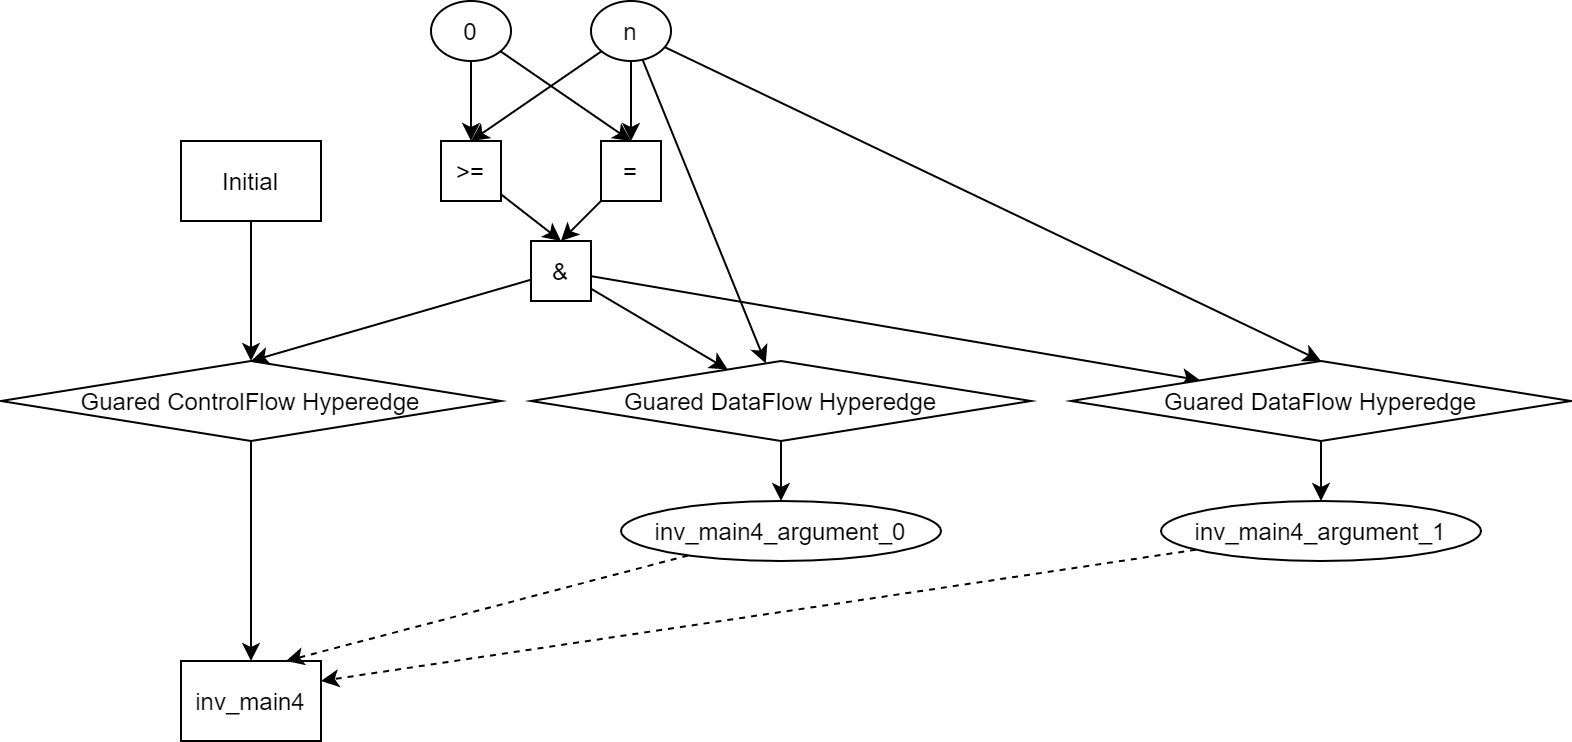
\includegraphics[width=14cm]{graph/horn-grapn-line-0}\\
  \caption{Horn graph for horn clause inv\_main4(x, y) :- ,[n >= 0 \& x = n \& 0 = n \& y = n]}\label{horn-grapn-line-0}
\end{figure}

In the similar way, Figure \ref{horn-grapn-line-1} illustrates how to draw Line 1 "inv\_main4(arg1, arg2) :- inv\_main4(x, y), [x != 0 \& x + -1 = arg1 \& y + -1 = arg2 \& n = 0]". Since $Head$ and $Body$ have the same control location node and arguments, control location node "inv\_main4" points to itself and guarded by a control flow hyperedge. arg1 is x and arg2 is y. They are drawn as inv\_main4\_argument\_0 and inv\_main4\_argument\_1 and connected to the control location node "inv\_main4". $Constrain$ [x != 0 \& x + -1 = arg1 \& y + -1 = arg2 \& n = 0] includes two $Guard$ n = 0, x != 0 and two $dataFlow$ x + -1 = arg1, y + -1 = arg2.

\begin{figure}[h]
\centering
  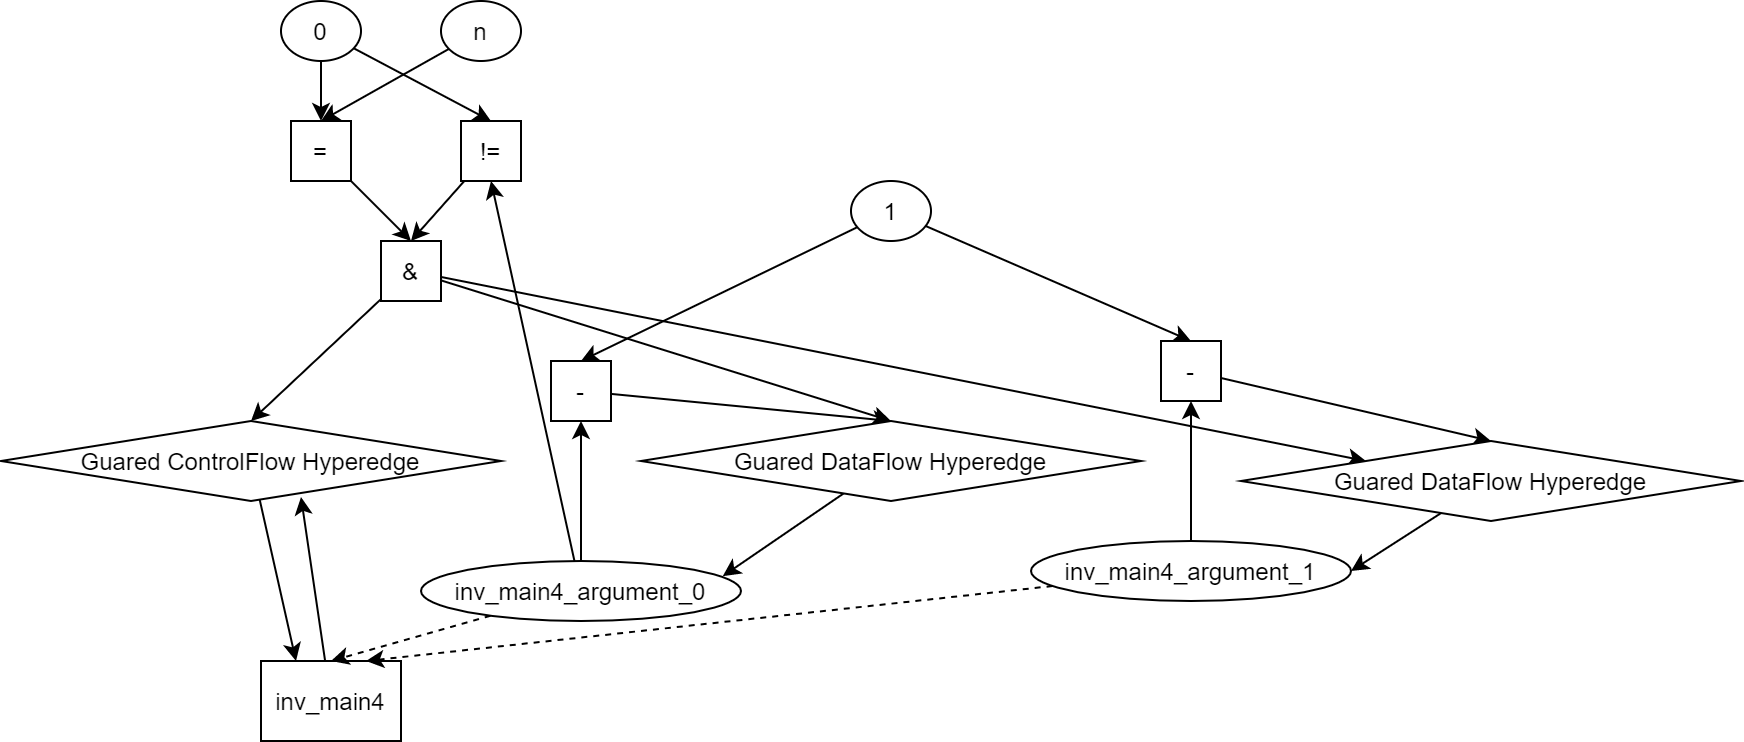
\includegraphics[width=14cm]{graph/horn-grapn-line-1}\\
  \caption{Horn graph for horn clause inv\_main4(arg1, arg2) :- inv\_main4(x, y), [x != 0 \& x + -1 = arg1 \& y + -1 = arg2 \& n = 0]}\label{horn-grapn-line-1}
\end{figure}

Figure \ref{horn-grapn-line-2} shows how to construct Line 2 "false :- inv\_main4(0, y), [y != 0]". We draw a connection from $Body$'s control location node "inv\_main4" to $Head$' control location node False $CL_{false}$. $Body$'s first argument (i.e. inv\_main4\_argument\_0) imply a data flow (inv\_main4\_argument\_0 $\leftarrow$ 0). This data flow is not from $Constrain$, so there is no guard for it. $Constrain$ [y != 0] is a $Guard$ because it is not a assignment operation. We know inv\_main4\_argument\_0 = 0 and inv\_main4\_argument\_1 = y, so we connect inv\_main4\_argument\_0 and inv\_main4\_argument\_1 with operator node != . Then we connect the root of $Guard$ (i.e. !=) to guarded hyperedges.

\begin{figure}[h]
\centering
  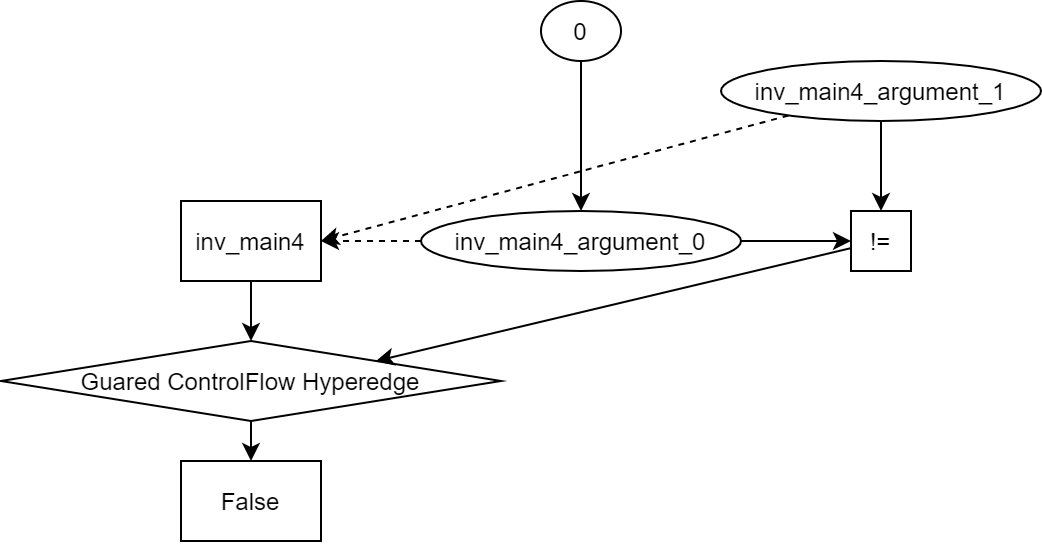
\includegraphics[width=8cm]{graph/horn-grapn-line-2}\\
  \caption{Horn graph for horn clause false :- inv\_main4(0, y), [y != 0]}\label{horn-grapn-line-2}
\end{figure}


A overview of the example horn graph construction is shown in Figure \ref{overall-transformation}

\begin{figure}[h]
\centering
  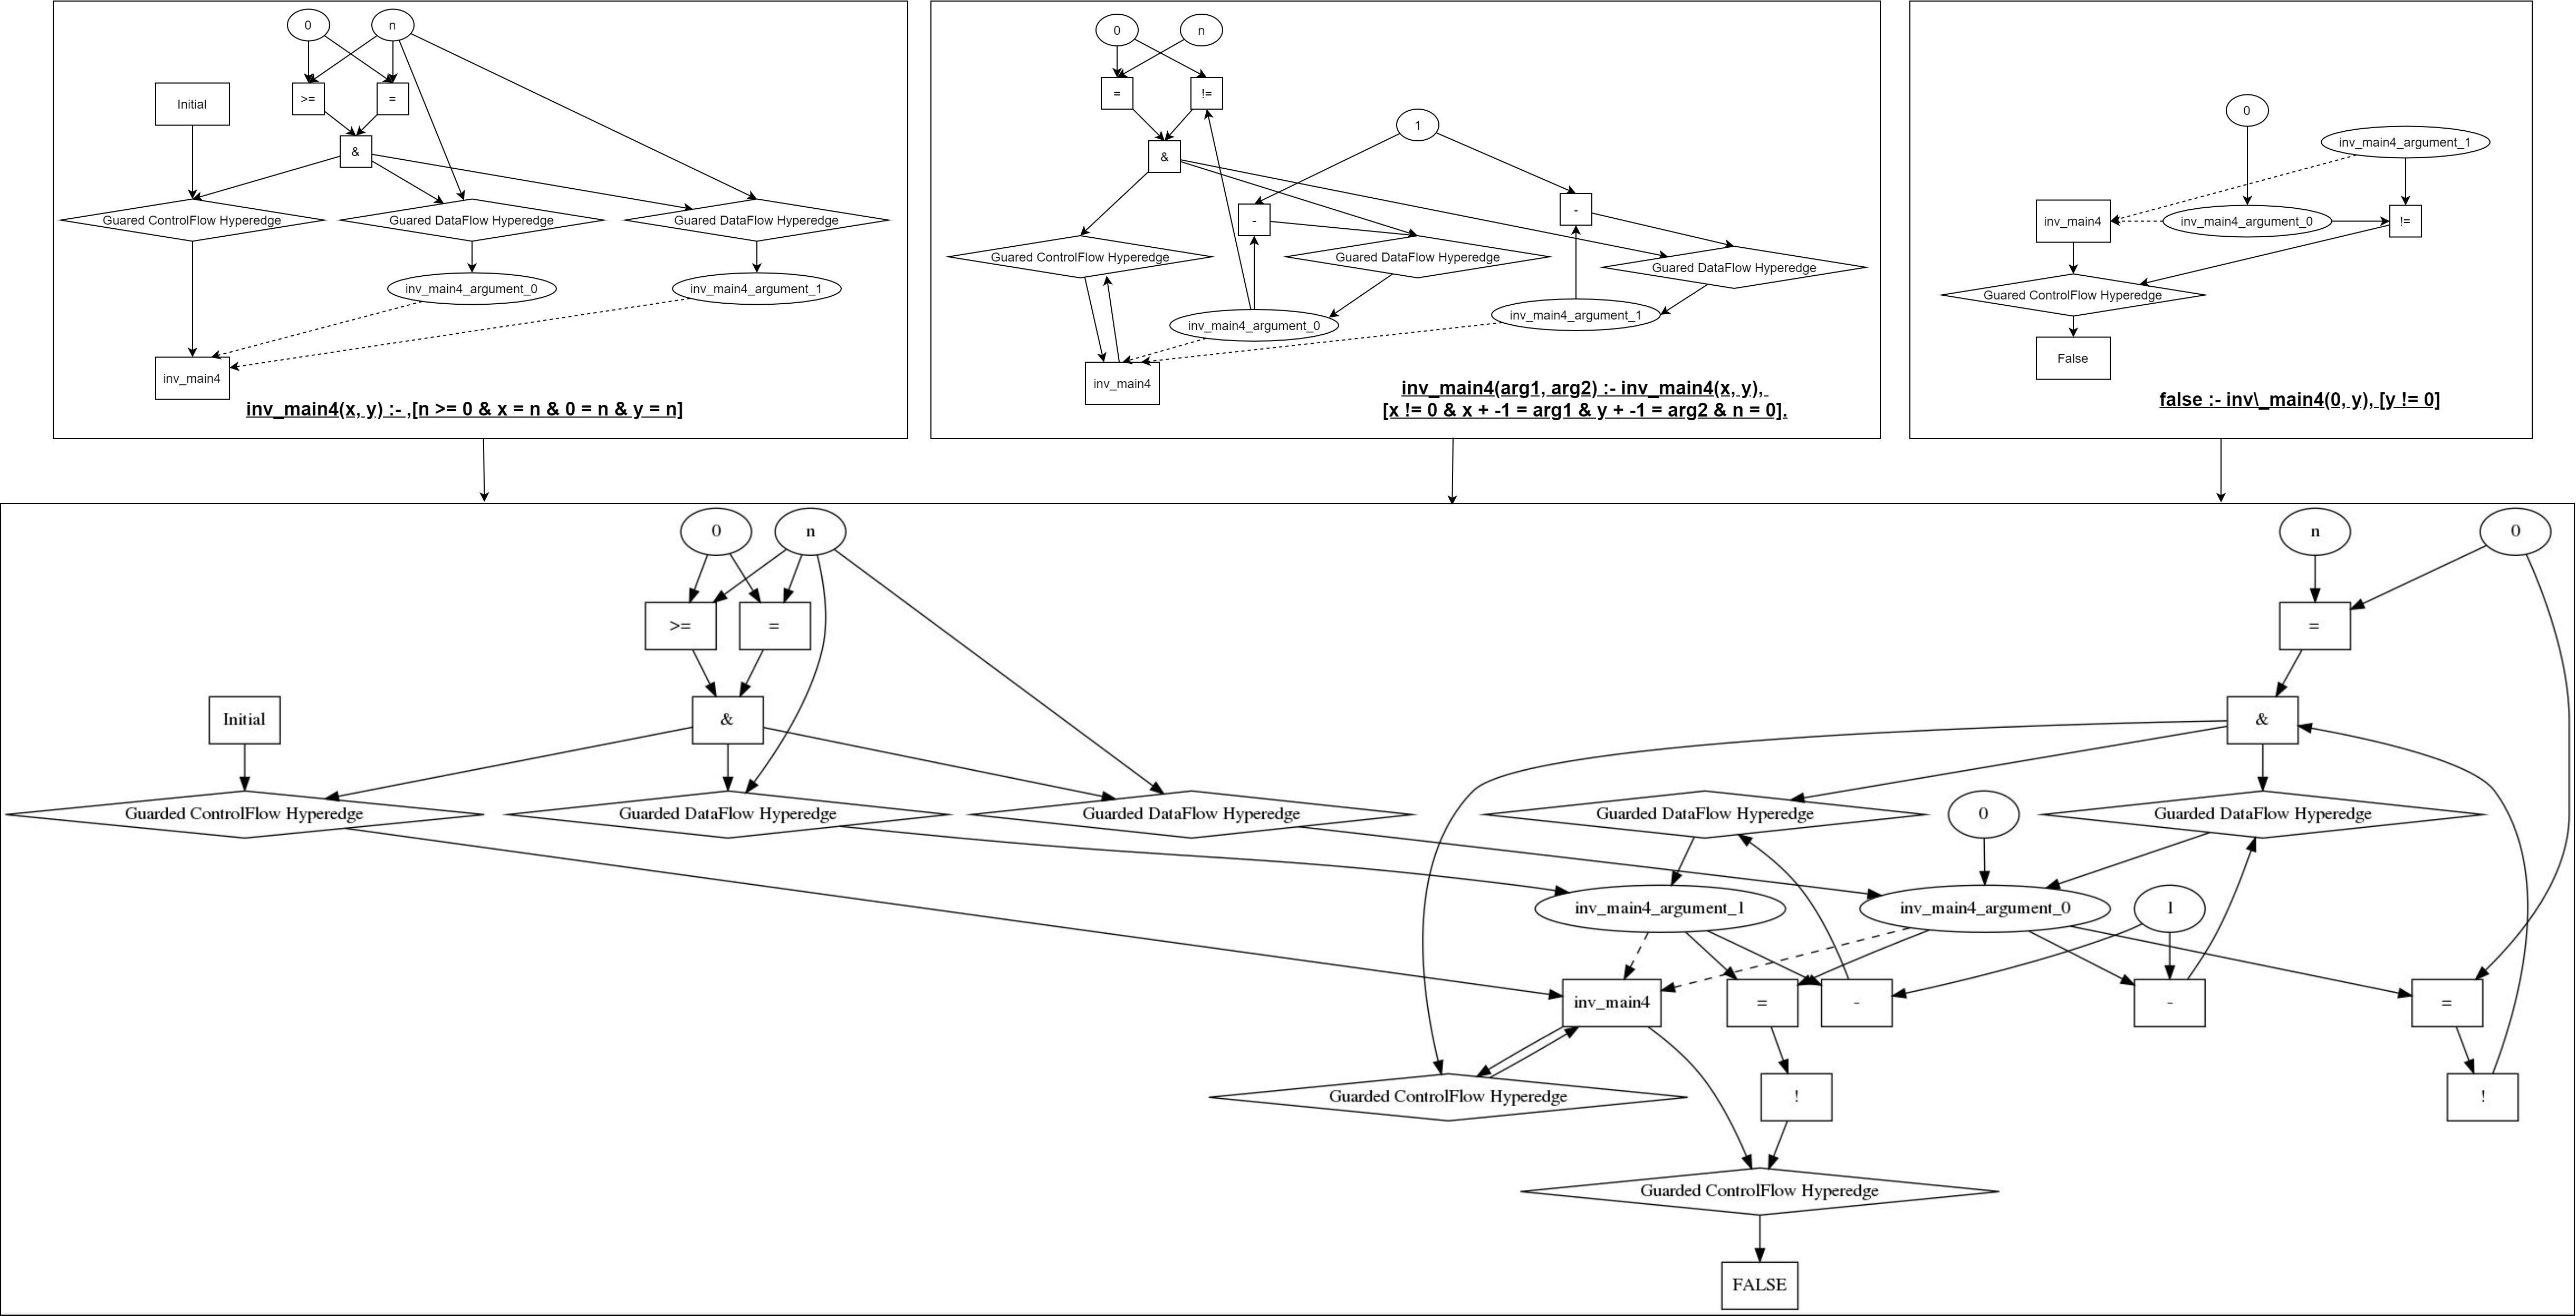
\includegraphics[width=16cm]{graph/overall-transformation}\\
  \caption{Overview of Horn graph construction for Figure \ref{while-C-horn-clauses}}\label{overall-transformation}
\end{figure}


\subsubsection{Horn graph Definition}



We first define all nodes and edges in the graph. Formally, the graph consists of four categories of nodes, two categories of hyperedges, and five categories of binary edges. The graph is defined as $G=(V_{CL},V_{Vri},V_{C},V_{Op},E_{CF},E_{DF},E_{CD},E_{Arg},E_{ST},HE_{CF},HE_{DF})$, in which $V_{CL}$ has three variance nodes $\{CL_{Initial},CL_{normal},CL_{false}\}$. They are control location nodes. $V_{Vri}$ is variable node, The variances are argument node $V_{arg}$ and free variable node$V_{free}$. $V_{C}$ is constant node. $V_{Op}$ is operator node which represents unary or binary operators.
$E_{CF}$ is control flow edge. It connects $V_{CL}$. $E_{DF}$ is data flow edge. It connect data flows to arguments. $E_{CD}$ is condition edge. It connects the root of $Guard$ through hyperedges to $V_{CL}$ and $V_{arg}$. The intuition is that all control flow and data flow are guarded by $Guard$ through hyperedges. $E_{ARG}$ is argument edge. It connect arguments to the corresponding control locations. The intuition is that the arguments belong to these control locations. $E_{ST}$ is syntax tree edge. All elements in syntax tree built by $Guard$ are connected by $E_{ST}$. $HE_{CF}$ is guarded control flow hyperedge. It connects $V_{CL}$ and guarded by the root of $Guard$ syntax tree. $HE_{DF}$ is guarded fata flow hyperedge. It connect all data flow elements from $V_{Vri}$ and $V_{C}$ to $V_{arg}$ guarded by the root of $Guard$ syntax tree as well.


%$V_{Arg}=\{Arg_{k}\}$ is argument set, $V_{C}$ is constant value set, $V_{Op}=\{+,-,==,...\}$ is operator set,$V_{FV}=\{v_{k}\}$ is free variables set. $k$ is a positive integer. $HE_{CF}$ is a set of Guarded control flow hyper edges. it is used between two control locations. it takes two inputs, a control location $cl_{Initial}$ or $cl_{Mian_{k}}$ and a boolean value from operator. It has a control flow out edge $e_{CFO}$ (one element from $E_{CFO}$) connected to next control location node. Similarly, $HE_{DF}$ is a set of Guarded data flow hyper edges. It guards the data flow from $Body$ to $Head$. It takes two inputs, a value from argument $Arg_{k}$ or free variable $v_{k}$ and a boolean value and has a data flow out edge $e_{DFO}$ (one element from $E_{DFO}$) connected to next operator or argument node. $E_{CFI},E_{CFO}$ are control flow in and control flow out edges, they are only used when there are connections between nodes and guarded control flow hyperedges. similarly, $E_{DFI},E_{DFO}$ are data flow in and out edges, they are only corresponding to guarded data flow hyperedges. $E_{CD}$ is condition edge. It connects boolean operator to the hyperedges to send boolean values to the hyperedges. $E_{Arg}$ is argument edge. It connects arguments to corresponding control location node. We use lower case to represent one elements in the set. For example $v_{CL}$ means one control location node from $V_{CL}$. $V_{Pred}$ is predicate node set. It connects the predicate's AST tree and the predicate's location.

The summary of $G$'s nodes and edges is shown in Table \ref{GraphDescriptionNodes} and \ref{GraphDescriptionEdges} respectively.
\begin{table}[h]\caption{Nodes in graph} \label{GraphDescriptionNodes}
\begin{center}
\begin{tabular}{lp{3cm}p{3cm}p{6cm}p{8cm}}
\hline
Graph Nodes & Name & Sub-elements & Connected edge types \\
\hline
$V_{CL}$  & Control location node            & $CL_{Initial}$, $CL_{normal}$, $CL_{false}$       & $E_{CF},HE_{CF}$\\
$V_{Vri}$ & Variable node                    & $V_{arg}, V_{free}$    & $E_{Arg},HE_{DF},E_{ST}$  \\
$V_{C}$   & Constant node                    & -                       & $E_{CF},E_{DF},E_{CD},E_{ST},HE_{CF},HE_{DF}$\\
$V_{Op}$  & Operator node                    & -                       & $E_{DF},E_{CD},E_{ST},HE_{CF},HE_{DF}$\\
\hline
\end{tabular}
\end{center}
\end{table}
%$V_{Pred}$ &Predicate node                   & Template types                                  & $v_{OP}$, $v_{Vri}$, $v_{C}$                      & $v_{CL}$ \\
\begin{table}[h]\caption{Edges in graph} \label{GraphDescriptionEdges}
\begin{center}
\begin{tabular}{lp{5cm}p{3cm}p{3cm}p{3cm}p{3cm}}
\hline
Graph Eedges & Name  & Start from & End at \\
\hline
%$E_{CFI}$ & Control flow in hyperedge                                               & $v_{CL}$   &$he_{CF}$\\
%$E_{CFO}$ & Control flow out hyperedge                                               &$he_{CF}$&$v_{CL}$\\
$E_{CF}$ & Control flow edge                                                    &$V_{CL}$ & $V_{CL}$\\
%$E_{DFI}$ & Data flow in hyperedge                                                     &$v_{OP}$, $v_{Arg}$, $v_{FV}$, $v_{C}$& $he_{DF}$\\
%$E_{DFO}$ & Data flow out hyperedge                                                    &$he_{DF}$ &$v_{OP},v_{Arg}$\\
$E_{DF}$ & Data flow edge                                                    &$V_{Vri},V_{C},V_{Op}$ & $V_{arg}$\\
$E_{CD}$ &  Condition edge                                                       &$V_{C},V_{OP}$ & $V_{CL},V_{arg}$\\
$E_{ARG}$ & Argument edge                                                        &$V_{Arg}$ & $V_{CL}$\\
$E_{ST}$ & Syntax tree edge                                                    &$V_{OP},V_{C},V_{Vri}$ & $V_{OP}$\\
$HE_{CF}$ & Guarded control flow hyperedge                                       & $V_{OP},V_{C}, V_{CL}$      & $V_{CL}$\\
$HE_{DF}$ & Guarded data flow hyperedge                                          & $V_{OP},V_{C},V_{Vri}$     & $V_{Arg}$\\
\hline
\end{tabular}
\end{center}
\end{table}





%$Body$ has same structure with $Head$.
%If $Head$ and $Body$ have the same control location, then they share the control location and arguments.
%
%The $Constraint$ contains the constraints to make the transition from $Body$ to $Head$ satisfiable. We parse it to two information, data flow AST and constraint AST.  Data flow AST takes $Body'$ arguments, constant value, or free variables in $constraint$ as inputs, and go through some arithmetic operator to the root as output (a value) eventually to an $Head'$ argument. The constraint AST takes $Body$' arguments, free variables in $constraint$ as the inputs. The root of the constraint AST tree is a boolean operator which can output a boolean value to all guarded control and data flow hyperedges from $Body$ to $Head$. If there is no $constraint$, the boolean value inputs to the hyperedges are set to true.

\textbf{Horn graph construction}.\\
We can represent the transition by $Head(V_{CL}^{Head},V_{arg}^{Head}):-Body(V_{CL}^{Body},V_{arg}^{Body}),[Constraint(Guard, DataFlow)]$.
We can construct the graph by following steps:

\begin{enumerate}
  \item We connect arguments to corresponding control locations in $Head$ and $Body$. $V_{arg}^{Head}$ connects to $V_{CL}^{Head}$ and $V_{arg}^{Body}$ connects to $V_{CL}^{Body}$ by $E_{ARG}$. If $V_{CL}^{Head} == V_{CL}^{Body}$ which implies $V_{arg}^{Head} == V_{arg}^{Body}$, only one set of arguments and corresponding control location nodes are drawn.
  \item We build the control flow by connecting control location node $V_{CL}^{Body}$ in $Body$  to control location node $V_{CL}^{Head}$ in $Head$ through guarded control flow hyperedge $HE_{CF}$. If $V_{CL}^{Head} == V_{CL}^{Body}$, it points to itself and also through $HE_{CF}$.
  \item In $Constraint$, we have two types of expressions (i.e. $Dataflow$ and $Guard$ ). If the expression is a assignment, and there are arguments involved, then it is a $Dataflow$, otherwise, it is a $Guard$. For $Dataflow$. We first draw a syntax tree(connected by $E_{ST}$) for the right hand side of the assignment expression . The root of the syntax tree connects to the left hand side argument through data flow hyperedge $HE_{DF}$. For $Guard$, we build a syntax tree (connected by $E_{ST}$) for it and connect the root to all $HE_{CF}$ and $HE_{DF}$ in this transition by $E_{CD}$. This means all control flow and data flow are guarded by $Guard$.
      If there is no $Guard$ in $Constraint$, a constant node with boolean value $True$ will be the root of $Guard$.
  \item $Head$ and $Body$ may imply some data flows. We can directly draw these data flows using $E_{DF}$. They are not guarded by $Guard$. The example can be found in previous Section \ref{Horn-graph-construction-example}
\end{enumerate}


%We can represent the transition by the definition of graph:
%
%$Head(CL_{Main_{m}},Arg_{head}):-Body(CL_{Main_{n}},Arg_{body}),[Constraint(Arg_{head},Arg_{body},V_{C},V_{Op},V_{FV})]$, where $m$ and $n$ are positive integer numbers. They can be equal or not equal. $Arg_{head}$ and $Arg_{body}$ are the set of arguments in head and body respectively. If $m==n$, $Arg_{head} == Arg_{body}$.
%
%To associate $Head$ and $Body$, we represent control flow information first by connecting the control location from $Body$ to $Head$, and between the control locations, there is a guarded control flow hyperedge which takes $Body$' control location and the boolean value from AST tree constructed from $constraint$ as inputs and output the control location information to $Head$'s control location. Then, we build data flow between $Head$ and $Body$. Every argument in $Head$ is guarded by a guarded data flow hyper edge which takes $Body$' arguments, data flow AST tree root, or free variables and the boolean value from $constraint$'s AST tree as inputs. In summary, all the control and data flows from $Body$ to $Head$ are guarded by a hyperedge, and one of the inputs of the hyperedges is the boolean value from the root of constraint AST tree constructed by the predicates in $constraint$.


%The constructed horn graph of a simple while loop program in Figure \ref{while-C-program} is shown in \ref{whileLoop-c-gv}. This graph is stored in .gv format and rended by dot engine.
%\begin{figure}[h]
%\centering
%  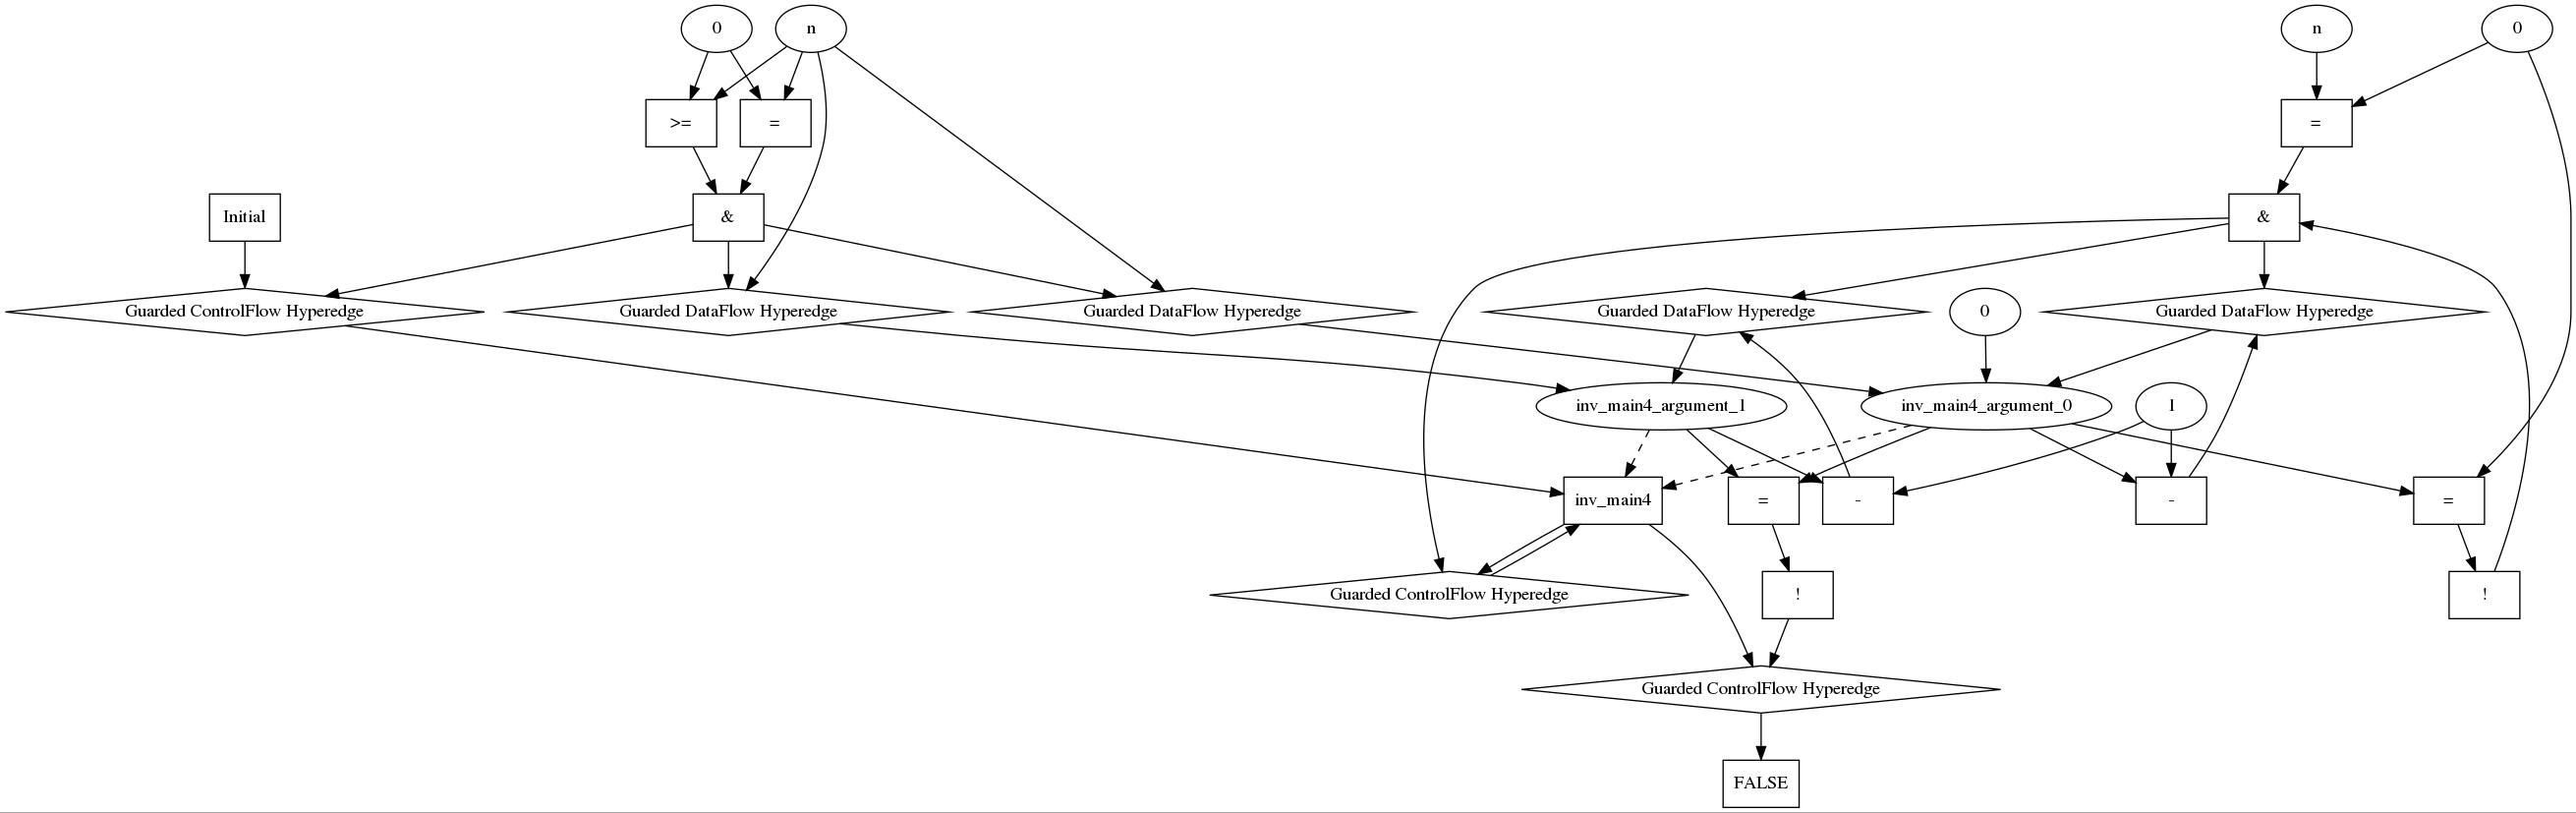
\includegraphics[width=16cm]{graph/whileLoop}\\
%  \caption{Training structure}\label{whileLoop-c-gv}
%\end{figure}






%\textbf{Graph Representation.}



%\subsection{Templates Representation}
%
%Each template contain location, category, and predicate information. One example template is "inv\_main8:VerifHintInitPred(((\_0 + -1 * \_2) >= 0))" in which "inv\_main8" is its control location,"VerifHintInitPred" is its category (The meaning of the categories can be found in appendix), and "(((\_0 + -1 * \_2) >= 0))" is the predicate. \_0 and \_2 are canonical encoding of variable names in source code. For example, \_0 is x and \_2 is y.  We can combine the three components into one graph. The root node contains the location information ("inv\_main8") as its node attribute. The only child of the root contains the category information ("VerifHintInitPred"). The predicate ("(((\_0 + -1 * \_2) >= 0))") can be represent as a binary tree. We connect the binary tree's root to the category node to connect all parts together. One example is shown in Figure \ref{templateGraph}. We use graphviz to manipulate the graph. The corresponding graphviz text representation of the template is shown in \ref{templateGraphviz}
%\begin{figure}[h]
%\centering
%\begin{subfigure}{0.3\textwidth}
%\begin{lstlisting}
%digraph dag {
%0 [label="inv_main8/4"];
%1 [label="VerifHintInitPred"];
%2 [label=">="];
%3 [label="0"];
%4 [label="+"];
%5 [label="_0"];
%6 [label="*"];
%7 [label="-1"];
%8 [label="_2"];
%0->1
%1->2
%2->4
%2->3
%4->6
%4->5
%6->8
%6->7
%\end{lstlisting}\subcaption{Template graph example in graphviz format}\label{templateGraphviz}
%\end{subfigure}   ~~~~~~~~~~~~
%\begin{subfigure}{0.3\textwidth}
%  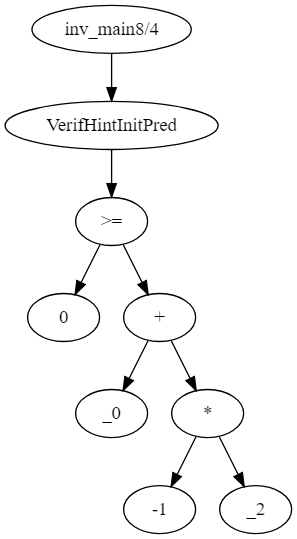
\includegraphics[width=3.4cm]{graph/template_graph}\\
%  \subcaption{Template graph example}\label{templateGraph}
%  \end{subfigure}
%  \caption{Graph representation for an example template "inv\_main8:VerifHintInitPred(((\_0 + -1 * \_2) >= 0))"}
%\end{figure}
%
%


\section{Data Collection}
Our raw inputs are programs in form of .smt2. The customized Eldarica can transform the program to horn clause, then draw horn graph and save the graph to dot format (.gv file). We transform horn graphs to standard GNN inputs (nodes vectors and edges). GNN can learn the node representation. We gather argument node representations from all node representations to be the input of the multilayer perceptron. The output (label) of the multilayer perceptron for each argument representation input is the number of occurrence of that argument node appeared in refined predicates. The multilayer perceptron is trained with GNN together.

The refined predicates are obtained from Algorithm \ref{Predicates-extracting-process} and described in next subsection.



\subsection{label collection}
All programs in benchmarks can be solved by Eldarica in a limited time. We feed these programs to Eldarica, then the CEGAR process will produce a set of predicates to build the abstract transition system (abstract model). But these predicates are redundant. We use Algorithm \ref{Predicates-extracting-process} to further refine the predicates. Then, we count the number of occurrence of arguments in these refined predicates to be our training labels. If there is no refined predicate found, then there is no label to be collected.

Algorithm \ref{Predicates-extracting-process} describes a single instance of predicates refining process, the inputs are a program in form of .smt2 and a list of initial templates $TemplateList=\{T_{0},T_{1},...,T_{n}\}$ crafted manually \cite{10.1007/978-3-319-57288-8_18} or generated by simple heuristics\cite{Leroux2016} . The program will be transformed to horn clauses ($HornClauses$). The templates are heuristics for predicates generating and generated before the CEGAR iteration. $TemplateList$ could be a empty list which means no heuristic for predicate generating. The output is a set of refined predicates $CriticalPredicateList$.

With these two inputs, we start the CEGAR process. We can get a list of predicates ($ExtractedPredicateList$) derived from $T$ and counter-examples in CEGAR iterations. If $ExtractedPredicateList$ is not empty, the predicates refining process begins. If $ExtractedPredicateList$ is empty, we don't need any predicate to verify the program. No label is extracted in this case.

We suppose there is no redundancy in $ExtractedPredicateList$ and assign $ExtractedPredicateList$ to $CriticalPredicateList$ before the refining process. Then, we delete predicates one by one from $CriticalPredicateList$ and see if we can verify the program with remaining predicates. To do so, we need a customized CEGAR $\widehat{CEGAR}$ which does not generate new predicates from counter-examples. In other words, $\widehat{CEGAR}$ will only use $CriticalPredicateList$ as initial predicates to build the abstract model.

If $\widehat{CEGAR}(HornClauses, CriticalPredicateList)$ returns False, which means $\widehat{CEGAR}$ cannot find the correct abstract model with remaining predicates within a fixed time, then we determine that the deleted one predicate is critical, and we add this back predicate to $CriticalPredicateList$. In the contrast, if $\widehat{CEGAR}(HornClauses, CurrentTemplateList)$ returns True, we don't add the predicate back to $CriticalPredicateList$.

By repetitively deleting predicate one by one from $CriticalPredicateList$, and check the solvability by $\widehat{CEGAR}$. We finally get a set of non-redundant predicates ($CriticalPredicateList$) that represents correct abstract model.

Notice that $ExtractedPredicateList$ may contain multiple $CriticalPredicateList$ that can represent correct abstract model in the fixed time. For example, $ExtractedPredicateList=\{P_{0},P_{1},P_{2}\}$. Both $\{P_{0},P_{1}\}$ and $\{P_{1},P_{2}\}$ can represent the abstract model correctly. This method only find one set of them. One can also first construct the permutation of $ExtractedPredicateList$, then use $\widehat{CEGAR}$ find all $CriticalPredicateList$. But, in the case of some complicated programs, there may be a large number of predicates in $ExtractedPredicateList$. Therefore, finding all $CriticalPredicateList$ is hard.


\begin{algorithm}[H]\label{Predicates-extracting-process}
\SetAlgoLined
\textbf{Input}:  TemplateList = $\{T_{0},T_{1},...,T_{n}\}$, HornClauses\;
\textbf{Output}: CriticalPredicateList \;
%\KwResult{$T_{0}^{l},T_{1}^{l},...,T_{n}^{l}$}
 ExtractedPredicateList=CEGAR(TemplateList,HornClauses)\;
 \eIf{ExtractedPredicateList is empty}{No CriticalPredicateList extracted}{

    CriticalPredicateList=ExtractedPredicateList\;
    \For{$P_{k}$ in ExtractedPredicateList}{
        CriticalPredicateList = CriticalPredicateList $ - \{P_{i}\} (i \in [0,n])$\;
        Solvalbility=$\widehat{CEGAR}$(CurrentPredicateList,HornClauses)\;
        \If{Solvalbility == False}{
            CriticalPredicateList = CriticalPredicateList $\cup$ $P_{i}$;\
        }
    }
    %Templates=transform(RedunantPredicateList $\cup$  CriticalPredicateList);\
 }

 \caption{Predicates refining process}
\end{algorithm}


%
%\begin{algorithm}[H]
%\SetAlgoLined
%\KwResult{$T_{0}^{l},T_{1}^{l},...,T_{n}^{l}$}
% initialization:  CurrentTemplateList = $\{T_{0},T_{1},...,T_{n}\}$\;
% Solvalbility=CEGAR(CurrentTemplateList,HornClauses)\;
%   \eIf{Solvalbility == True}{
%    \While{CurrentTemplateList is not empty}{
%        CurrentTemplateList = CurrentTemplateList $ - \{T_{k}\} (0\leqslant k \leqslant n)$\;
%        Solvalbility=CEGAR(CurrentTemplateList,HornClauses)\;
%        \eIf{Solvalbility == True}{
%            RedunantTemplateList=RedunantTemplateList $\cup$ $T_{k}^{0}$;\
%        }{
%            CriticalTemplateList=CriticalTemplateList $\cup$ $T_{k}^{1}$;\
%        }
%        Templates=RedunantTemplateList $\cup$  CriticalTemplateList;\
%    }
%   }{
%   Cannot solve within timeout, no template extracted\;
%  }
% \caption{Templates extracting process}
%\end{algorithm}

%The output is a list of templates with 0 or 1 labels $T_{0}^{l},T_{1}^{l},...,T_{n}^{l}, l= 0$ or $1$. A concrete example for an output is $T_{0}^{1} = ("inv\_main8:VerifHintInitPred(((\_0 + -1 * \_2) >= 0))",1)$

%The final goal is to have proper predicates that can represent the abstract transition system. The templates are heuristics to generate the predicates in each CEGAR iteration. There are additional predicates added to solve the program in every CEGAR iterationl but the templates are given and fixed before the CEGAR iteration.

%The strategy $A$ (fixed time out) to extract the training data (a list of templates with labels) is that for one program, we run Eldarica with an abstraction heuristic (e.g. use option -abstract:manual for .c files and -abstract for .smt2 files). If Eldarica can solve the program within 60 seconds. We mark this program as solvable. In Eldarica, we have an initial list of templates. We delete these templates one by one to see if the program can be solved with the remaining templates. If the program is still solvable within the timeout, then that deleted template is critical, we mark it as useful and label it as 1. By doing so iteratively, we can label the initial list of templates. This labelled list of templates will be used in the training process.
%
%\begin{enumerate}
%  \item chc-comp benchmarks: 38/1216 .smt2 files (programs) need templates to solve the program within in 60 seconds.
%  \item sv-comp smt benchmarks: 7/6814 .smt2 files need templates.
%  \item sv-comp c benchmarks: 31/545 .c files need templates.
%\end{enumerate}
%
%Only 76 training programs in total.

%Extracting data with variable timeout: First, confirm the solvability (i.e. the program can be solved within 60 seconds with the abstraction heuristic).
%Second, record the solving time with and without the abstraction heuristic. If Eldarica takes less solving time with abstraction heuristic, pass this solving time as timeout to Eldarica to label the templates used in the program.






%
%\begin{enumerate}
%  \item chc-comp benchmarks: 40/1216.  32 programs (204 templates)for training and 8 (47 templates) for testing. 8/8 solved by read templates. Read templates time consumption/original templates consumption =  40.25/40.86 (in seconds)
%  \item sv-comp smt benchmarks: 15/5911.  12 programs (254 templates)for training and 3 (74 templates) for testing. 3/3 solved by read templates. Read templates time consumption/original templates consumption =  28.07/27.28 (in seconds)
%  \item sv-comp c benchmarks: 41/555.  32 programs (4635 templates)for training and 9 (350 templates) for testing. 8/9 solved by read templates. Read templates time consumption/original templates consumption = 34.04/53.46  (in seconds)
%\end{enumerate}
%
%96 training programs. 76 programs for training, 20 programs for testing.
%18/20 solved by read templates. Read templates time consumption/original templates consumption =  140.67/126.84 (in seconds)
%
%Extracting data on larger benchmarks, and use these three benchmarks only for testing.


%We try to use balanced and imbalanced data set to train the neural network.



%\begin{table}
%\begin{center}\caption{Balanced Predicates}
%\begin{tabular}{lp{1.5cm}p{2cm}p{2cm}p{1.5cm}p{1.5cm}p{1.5cm}p{1.5cm}p{1.5cm}}
%\hline
%Benchmarks  & Training program &Testing program&Training  predicates & Testing predicates & Solved programs & Time consumption(predicated/abstract)\\
%\hline
%chc-comp-smt  &133/167&34/167&700/1174&474/1174& 34/34 & 105.4/105.2\\
%sv-comp-smt  &-&-&-&-\\
%sv-comp-c  &148 & 30 & 1482 & 1128& 23/30 & 3608&7796\\
%In total &-&-&-&-\\
%\hline
%\end{tabular}
%\end{center}
%\end{table}

%\subsection{Argument labelling}
%After we separate templates according to their usefulness, for every argument in a location, we count the occurrence in useful templates in that location to be argument's score which is the training label.

\section{Learning Model}
The learning model is shown in Figure \ref{training-framework}. The input horn graph is transformed from a program by Eldarica. For a horn graph, we transform the node to vectors by embedding layer. The edges include relation between node vectors. GNN takes node features and their relations (edges) as inputs. It outputs node embeddings. Then, we gather argument node embeddings $v_{argument~node}'$ to be the inputs of multilayer perceptron. The final outputs are the number occurrences of arguments appeared in refined predicates. GNN and the multilayer perceptrons are trained together.

\begin{figure}[h]
\centering
  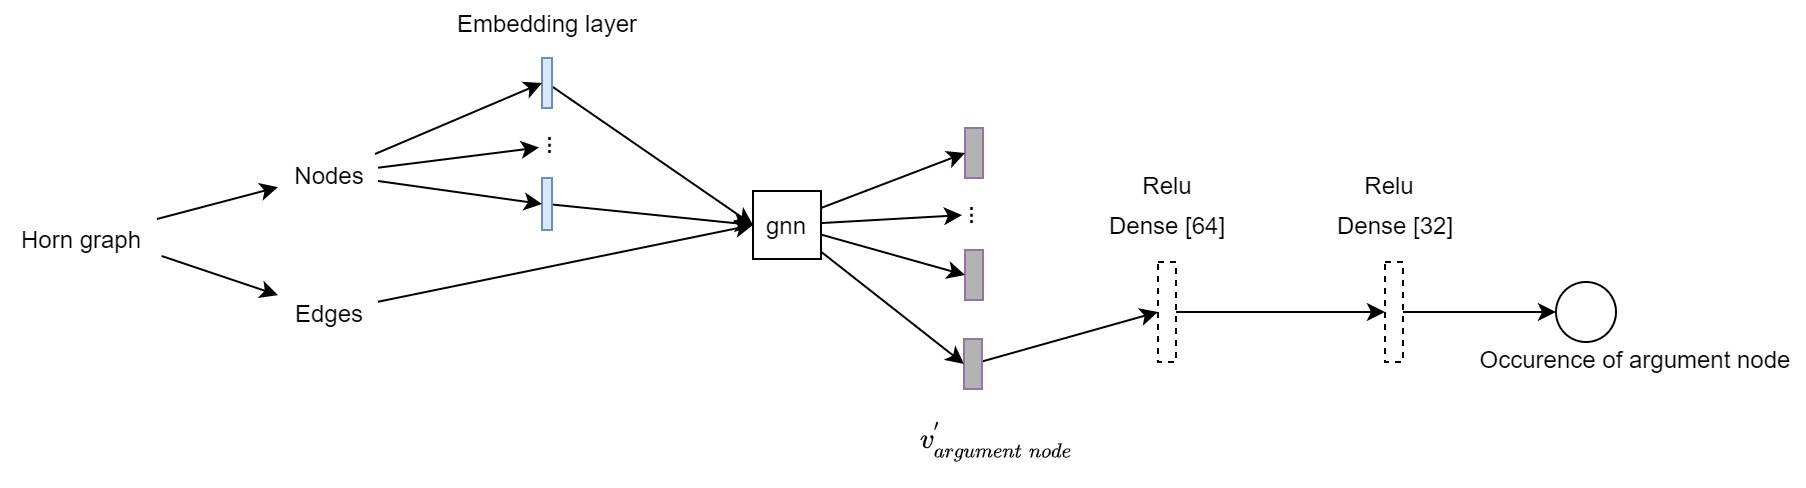
\includegraphics[width=16cm]{graph/training-framework}\\
  \caption{Training structure}\label{training-framework}
\end{figure}

\subsection{Training results and analysis}
We collected the number of arguments' occurrence to be our training label. Since we care about the importance of the arguments, we can transform the occurrence label to ranking and learn the ranking of arguments. So we have two variances of our training. One is to predict the occurrence using occurrence label directly, then rank the predicted number or normalize them to represent the importance and feed back to Eldarica. Another variance is to predict the ranking using ranking label.

The numerical results of training using different labels are shown in \ref{training-results}
\begin{table}[h]\caption{Training results}\label{training-results}
\begin{center}
\begin{tabular}{lp{1.5cm}p{1.5cm}p{1.5cm}p{1.5cm}p{1.5cm}p{1.5cm}p{1.5cm}p{1.5cm}}
\hline
Benchmarks  & Label & Train loss & Valid loss & Test loss & Mean loss & Best valid epoch  \\
\hline
LIA-lin       & occurrence & 0.003 & 0.548 & 20.603 & 20.848 & 8 \\
LIA-lin       & rank & 0.0002 & 0.0092 & 3.194 & 0.684 & 52 \\
LIA-nonlin    & occurrence & - & - & - & - & - \\
LIA-nonlin    & rank & - & - & - & - & - \\
In total      & occurrence & - & - & - & - & - \\
In total      & rank & - & - & - & - & - \\
\hline
\end{tabular}
\end{center}
\end{table}

Parameters: max\_epochs=1000,patience=50, Node dimension=64. MLP=[64x64]...




Graph analysis:

\begin{table}[h]\caption{Benchmark analysis}\label{training-results}
\begin{center}
\begin{tabular}{lp{2cm}p{2.5cm}p{2.5cm}p{2.5cm}p{2.5cm}p{1.5cm}p{1.5cm}p{1.5cm}}
\hline
Benchmarks  & Average argument quantity[range] & Average argument occurrence & Average node quantity & Average binary edge quantity & Average ternary edge quantity  \\
\hline
LIA-lin (train)     & 31.59 [1,796] & 2.27[0.01,116.66] & 1070.25[14,31264] & 1514.30[12,50849] & 401.90[5,4309]\\
LIA-lin (valid)     & 25.21[1,330] & 1.31[0.01,8.75] & 877.71[21,12320] & 1213.35[18,16315] & 297.59[5,3966]  \\
LIA-lin (test)     & 16.86[2,311] & 3.40[0.03,76.5] & 1096.42[20,19371] & 1512.16[15,27723] & 324.10[7,5665]  \\
\hline
\end{tabular}
\end{center}
\end{table}






%\begin{figure}[h]
%\centering
%  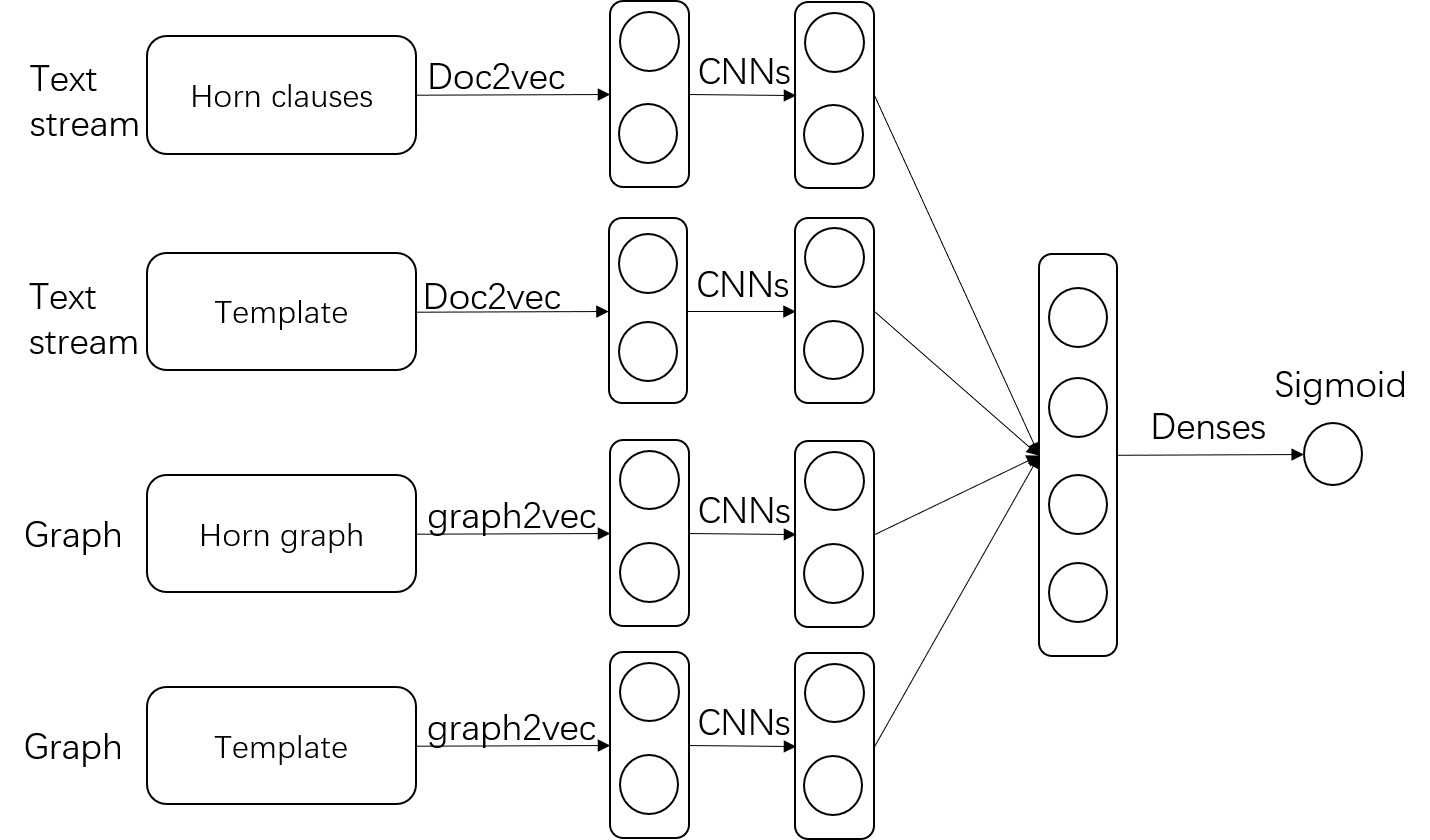
\includegraphics[width=10cm]{graph/NNstructure}\\
%  \caption{Neural network structure}\label{NNstructure}
%\end{figure}
%\subsection{Program Embedding}
%
%\subsubsection{Text Level}
%Doc2Vec \cite{DBLP:journals/corr/LeM14} embed different length of sentences to fixed vector.
%Program text streams are embedded into 100 dimensions. Template text streams are embedded to 20 dimensions.
%\subsubsection{Graph Level}
%Graph2Vec\cite{DBLP:journals/corr/NarayananCVCLJ17}.
%WL relabeling process \cite{WL_relabeling_process} to generate random subgraphs (can be seen as sentences). Then use Doc2Vec embed subgraphs to fixed vector.
%Program graphs (horn graphs) are embedded into 100 dimensions. Templates are embedded to 20 dimensions.



%\section{Experiments}
%The predicted result is a score for a template. We add two rank modes to decide which templates will be used for solving a particular program. For example, we have 10 templates, their scores ranged from 0 to 1. The first rank mode can specify a threshold for the scores. If the threshold is 0.4, all templates that have scores larger than 0.4 will be used to solve the program, and the left templates are discarded. The second rank mode can specify a hierarchical number (N) which decides to use top N ranked templates by score. If we specify the hierarchical number (N) be 5, then the top 5 ranked templates by score will be used to solve the program, and the left 5 templates will be discarded.


\section{Feed learned heuristic back to Eldarica}

\section{Evaluation}
\subsection{Benchmarks}

We separate our benchmarks to linear or nonlinear group. All programs in the benchmarks can be verified by Eldarica in a limited time.
In these verifiable programs, we use Algorithm \ref{Predicates-extracting-process} to select programs that need initial predicates to be verified. Then we transform these selected programs to horn graphs and divide them to train, valid, and test set randomly. The numerical details can be found in Table \ref{benchmark-train-valid-test}

\begin{table}[h]\caption{Benchmarks}\label{benchmark-train-valid-test}
\begin{center}
\begin{tabular}{lp{2cm}p{3cm}p{2cm}p{2cm}p{2cm}}
\hline
Benchmarks  & Total program & Graphs with labels & Train & Valid & Test  \\
\hline
LIA-lin       & 7741 (7533)  & 413 & 247 & 82 & 84 \\
LIA-nonlin    & 7653         & 1212 & 727 & 242 & 243 \\
In total      & 15394(15186) & 1625 & 974 & 324 & 327 \\
\hline
\end{tabular}
\end{center}
\end{table}

\subsection{Setup}

Eldarica settings:
Timeout for verifying a program.

learning model settings:
R-GCN.



All code regarding the experiment can be found in Git repository \href{https://github.com/ChenchengLiang/Systematic-Predicate-Abstraction-using-Machine-Learning}{https://github.com/ChenchengLiang/Systematic-Predicate-Abstraction-using-Machine-Learning}

\subsection{Experimental results}

\begin{table}[h]
\begin{center}
\begin{tabular}{lp{2cm}p{2cm}p{3.5cm}p{3cm}}
\hline
Benchmarks  & Total program  & No heuristic & Templates as heuristic & Learned heuristic\\
\hline
LIA-lin    & - & -&-&-\\
LIA-nonlin & - & -&-&-\\
Total  & - & -&-&-\\
\hline
\end{tabular}\caption{The number of verified programs in fixed time}
\end{center}
\end{table}

\begin{table}[h]
\begin{center}
\begin{tabular}{lp{3cm}p{3cm}p{3cm}p{3cm}p{3cm}p{3cm}p{3cm} }
\hline
Benchmarks  & Average CEGAR iterations (No heuristic) & Average time consumption (No heuristic) & Average CEGAR iterations (learned heuristic) & Average time consumption (learned heuristic) \\
\hline
LIA-lin  & - & - & -&-\\
LIA-nonlin  & - & - & -&-\\
Total  & - & - & -&-\\
\hline
\end{tabular}\caption{Average CEGAR iterations and time consumption}
\end{center}
\end{table}
%
%
%
%\subsection{Ablation studies}
%
%
%
%\begin{table}\caption{Benchmarks}
%\begin{center}
%\begin{tabular}{lp{1cm}p{1cm}p{1.5cm}p{1.5cm}p{1.5cm}p{1.5cm}p{1.5cm}p{1.5cm}}
%\hline
%Benchmarks & File type & Total file & Solved & sat & unsat & Unsolved  \\
%\hline
%chc-comp-smt & .smt2 & 1216 & 421  & 339  & 82    & 795 \\
%sv-comp-smt &.smt2   & 5911 & 4730 & 4516 & 214  & 1181 \\
%sv-comp-c &.c        & 555  & 323  & 262  & 61   & 231 \\
%In total  & - & - & -&-&-&-&-&-\\
%\hline
%\end{tabular}
%\end{center}
%\end{table}
%
%
%\begin{table}[h]
%\begin{center}\caption{Imbalanced Predicates with control flow and template graph}
%\begin{tabular}{lp{1.5cm}p{2cm}p{2cm}p{1.5cm}p{1.5cm}p{2.5cm}}
%\hline
%Benchmarks  & Training program &Testing program&Training  predicates & Testing predicates & Solved programs & Total time consumption (predicted:abstract)\\
%\hline
%chc-comp-smt  & 130 & 33& 969 & 225 & 33/33 & 63.92 : 63.72 (s)\\
%sv-comp-smt  &784 &196 & 5907 & 1406 & 196/196 & 514.60 : 511.186 \\
%sv-comp-c  &116 & 29  & 4148 & 847 & 20/29 &  578.33 : 56.74  \\
%In total  & 1030 & 258 & 10588 & 2914 & 250/258 & 1119.73 : 629.82 \\
%\hline
%\end{tabular}
%\end{center}
%\end{table}
%
%
%\begin{table}[h]
%\begin{center}\caption{Imbalanced Templates with control flow and template graph}
%\begin{tabular}{lp{1.5cm}p{2cm}p{2cm}p{1.5cm}p{1.5cm}p{2.5cm}}
%\hline
%Benchmarks  & Training program &Testing program&Training  predicates & Testing predicates & Solved programs & Time consumption (predicted/abstract)\\
%\hline
%chc-comp-smt  &- &- &- & - & - & - (s)\\
%sv-comp-smt  &-&-&-&-&-&-\\
%sv-comp-c  &- &- & - &-&-&-\\
%In total &-&-&-&-\\
%\hline
%\end{tabular}
%\end{center}
%\end{table}
%
%
%
%
%
%
%CEGAR iterations:
%
%Solvability:
%\begin{center}
%\begin{tabular}{lp{1cm}p{1cm}p{1cm}p{1cm}p{1cm}p{1cm}p{1cm} }
%\hline
%Benchmarks  & Total file & with template graph & with horn graph & with control flow graph &with control flow and template graphs & with horn and template graphs\\
%\hline
%chc-comp-smt & 1216 & -&-\\
%sv-comp-smt & 5911 & -&-\\
%sv-comp-c  & 555 & -&-\\
%\hline
%\end{tabular}
%\end{center}
%
%Time consumption:
%\begin{center}
%\begin{tabular}{lp{1cm}p{1cm}p{1cm}p{1cm}p{1cm}p{1cm}p{1cm} }
%\hline
%Benchmarks  & Total file & with template graph & with horn graph & with control flow graph &with control flow and template graphs & with horn and template graphs\\
%\hline
%chc-comp-smt  & 1216 & -&-\\
%sv-comp-smt  & 5911 & -&-\\
%sv-comp-c  & 555 & -&-\\
%\hline
%\end{tabular}
%\end{center}

\section{Related work}

DeepMath \cite{NIPS2016_6280} is the first trial that perform text-level learning to Guide formal method's search process. They use neural sequence models to select premises for automated theorem prover (ATP). Their input pair for the learning model is character-level or word-level conjecture and axiom. Output is the relevance of these two inputs. With the predicted relevances (range [0,1]), a importance rank of a set of axioms to one conjecture is obtained. DeepMath treats conjecture and axiom as text-level information and builds character-level and word-level models to embed them.

FormulaNet \cite{NIPS2017_6871} performs the same task (premise selection for theorem proving) like DeepMath. But, FormulaNet represent represent the input (a higher-order logic formula) as a graph and provide a embedding method to catch the formula's representation.

Our input is program.  Graph is a natural way to represent programs. There are different ways to learn the program graphs.

(1) End-to-end learning: TBCNN \cite{DBLP:journals/corr/MouLJZW14} takes AST as input and propose a tree-based convolutional neural network to learn program representation. \textit{Learning to represent programs with graphs} \cite{DBLP:journals/corr/abs-1711-00740} define a program graph based on AST to catch syntactic and semantic structure. Then, it uses GNN to learn the program representation.

(2) Semi-supervised or unsupervised graph embedding aims at using various methods to represent the graph to low-dimensional vector for down stream applications (e.g. classification, recommendation, etc.). The graph embedding and downstream networks are not trained jointly.
Before combining with deep learning, graph embedding works in the context of dimensionality reduction.
The typical techniques are principle component analysis (PCA), multidimensional scaling (MDS),Isomap \cite{Isomap}, Locally Linear Embedding (LLE) \cite{Roweis2323}, and Laplacian Eigenmap \cite{NIPS2001_1961}. Their complexities are quadratic corresponding to the number of vertices. DeepWalk \cite{DBLP:journals/corr/PerozziAS14} maps the graph's nodes to sentence's words and uses word embedding technique skip-gram \cite{DBLP:journals/corr/MikolovSCCD13} to perform the node embedding. And, it is extended to Graph2Vec \cite{DBLP:journals/corr/NarayananCVCLJ17} to learn the graph representation.
%
%
%Graph neural networks (GNNs) are deep learning model for graph-related task in end-to-end manner. The first state of nodes are given. Update node representations by edges type and the connected node.
%The edges, hyper-edges, messages should capture the characteristics or relations between nodes.
%
%
%Program graph representation.
%
%Graph neural networks (GNNs) are deep learning model for graph-related task in end-to-end manner. Message passing, convolutional graph neural network.
%Define a the first state of nodes. Update node representations by edges type and the connected node. Iteration is intuitively the filters of CNNs.
%The edges, hyper-edges, messages should capture the characteristics or relations between nodes.
%To deal with arbitrary length of information (different number of nodes), aggregation or abstraction then aggregation.
%
%AST embedding: code2vec \cite{Alon:2019:CLD:3302515.3290353}. TBCNN \cite{DBLP:journals/corr/MouLJZW14}.Learning to represent programs with graphs\cite{DBLP:journals/corr/abs-1711-00740}.
%
%
%FormulaNet \cite{NIPS2017_6871}. GAT \cite{2017arXiv171010903V}.

%Semi-supervised or unsupervised graph embedding aims at using various methods to represent the graph to low-dimensional vector for down stream applications (e.g. classification, recommendation, etc.). The graph embedding and downstream networks are not trained jointly.
%Before combining with deep learning, graph embedding works in the context of dimensionality reduction.
%The typical techniques are principle component analysis (PCA), multidimensional scaling (MDS),Isomap \cite{Isomap}, Locally Linear Embedding (LLE) \cite{Roweis2323}, and Laplacian Eigenmap \cite{NIPS2001_1961}. Their complexities are quadratic corresponding to the number of vertices.

%DeepWalk maps the graph's nodes to sentence's words and uses word embedding technique skip-gram to perform the node embedding. along with skip-gram word embedding later on been extended to Doc2Vec, DeepWalk node embedding is extended to Graph2Vec.
%The idea of Skip-gram word embedding later on is used in Doc2Vec,

%code2vec \cite{Alon:2019:CLD:3302515.3290353}
%Program synthesis:
%
%Logical reasoning: NEO, BLAZE, CEGIS.
%
%Machine learning methods:
%Program synthesis from examples:
%Encode inputs to fixed vector, then decode this vector to target language.
%
%Program induction:
%Directly give output. The learned program is induced latently within the weights and activations of a neural network.
%
%Guide formal method's search process by Training a statistical model to rank some options existed in search space and try them first.


\section{Discussion and Future work}
%
%
%\section{Headings: first level}
%\label{sec:headings}
%
%\lipsum[4] See Section \ref{sec:headings}.
%
%\subsection{Headings: second level}
%\lipsum[5]
%\begin{equation}
%\xi _{ij}(t)=P(x_{t}=i,x_{t+1}=j|y,v,w;\theta)= {\frac {\alpha _{i}(t)a^{w_t}_{ij}\beta _{j}(t+1)b^{v_{t+1}}_{j}(y_{t+1})}{\sum _{i=1}^{N} \sum _{j=1}^{N} \alpha _{i}(t)a^{w_t}_{ij}\beta _{j}(t+1)b^{v_{t+1}}_{j}(y_{t+1})}}
%\end{equation}
%
%\subsubsection{Headings: third level}
%\lipsum[6]
%
%\paragraph{Paragraph}
%\lipsum[7]
%
%\section{Examples of citations, figures, tables, references}
%\label{sec:others}
%\lipsum[8] \cite{kour2014real,kour2014fast} and see \cite{hadash2018estimate}.
%
%The documentation for \verb+natbib+ may be found at
%\begin{center}
%  \url{http://mirrors.ctan.org/macros/latex/contrib/natbib/natnotes.pdf}
%\end{center}
%Of note is the command \verb+\citet+, which produces citations
%appropriate for use in inline text.  For example,
%\begin{verbatim}
%   \citet{hasselmo} investigated\dots
%\end{verbatim}
%produces
%\begin{quote}
%  Hasselmo, et al.\ (1995) investigated\dots
%\end{quote}
%
%\begin{center}
%  \url{https://www.ctan.org/pkg/booktabs}
%\end{center}
%
%
%\subsection{Figures}
%\lipsum[10]
%See Figure \ref{fig:fig1}. Here is how you add footnotes. \footnote{Sample of the first footnote.}
%\lipsum[11]
%
%\begin{figure}
%  \centering
%  \fbox{\rule[-.5cm]{4cm}{4cm} \rule[-.5cm]{4cm}{0cm}}
%  \caption{Sample figure caption.}
%  \label{fig:fig1}
%\end{figure}
%
%\subsection{Tables}
%\lipsum[12]
%See awesome Table~\ref{tab:table}.
%
%\begin{table}
% \caption{Sample table title}
%  \centering
%  \begin{tabular}{lll}
%    \toprule
%    \multicolumn{2}{c}{Part}                   \\
%    \cmidrule(r){1-2}
%    Name     & Description     & Size ($\mu$m) \\
%    \midrule
%    Dendrite & Input terminal  & $\sim$100     \\
%    Axon     & Output terminal & $\sim$10      \\
%    Soma     & Cell body       & up to $10^6$  \\
%    \bottomrule
%  \end{tabular}
%  \label{tab:table}
%\end{table}
%
%\subsection{Lists}
%\begin{itemize}
%\item Lorem ipsum dolor sit amet
%\item consectetur adipiscing elit.
%\item Aliquam dignissim blandit est, in dictum tortor gravida eget. In ac rutrum magna.
%\end{itemize}


\bibliographystyle{unsrt}
%\bibliography{references}  %%% Remove comment to use the external .bib file (using bibtex).
%%% and comment out the ``thebibliography'' section.

\bibliography{references}
%%% Comment out this section when you \bibliography{references} is enabled.
%\begin{thebibliography}{1}
%
%\bibitem{kour2014real}
%George Kour and Raid Saabne.
%\newblock Real-time segmentation of on-line handwritten arabic script.
%\newblock In {\em Frontiers in Handwriting Recognition (ICFHR), 2014 14th
%  International Conference on}, pages 417--422. IEEE, 2014.
%
%\bibitem{kour2014fast}
%George Kour and Raid Saabne.
%\newblock Fast classification of handwritten on-line arabic characters.
%\newblock In {\em Soft Computing and Pattern Recognition (SoCPaR), 2014 6th
%  International Conference of}, pages 312--318. IEEE, 2014.
%
%\bibitem{hadash2018estimate}
%Guy Hadash, Einat Kermany, Boaz Carmeli, Ofer Lavi, George Kour, and Alon
%  Jacovi.
%\newblock Estimate and replace: A novel approach to integrating deep neural
%  networks with existing applications.
%\newblock {\em arXiv preprint arXiv:1804.09028}, 2018.
%
%\end{thebibliography}


\end{document}
